\clearpage
\section{Realisierung Gehäuse}\label{sec:Realisierung Gehäuse}
Im folgenden Teil des Fachberichtes ist die Realisierung des Gehäuse beschrieben. 

Die Anforderungen an das Gehäuse des digitalen Theremin sind:
\begin{itemize}
	\item Die Lautstärke- und die Tonhöhenantenne müssen genügend Abstand zueinander haben, damit der Spieler das Theremin richtig spielen kann.
	\item Das Antennenoszillator PCB und das DE1-SoC Board müssen für den Spieler ersichtlich sein.
	\item Für die Bedienung muss das LT24 Touch Modul für den Benutzer gut sichtbar platziert sein.
	\item Um den Preis des Gehäuses tief zu halten und für die Gestaltung des Gehäuses möglichst viel Freiheit zu haben, soll das Gehäuse 3D-gedruckt sein.  
\end{itemize}

Um diese Anforderungen zu erfüllen entschiedenen wir uns das Gehäuse mit dem 3D-CAD-System Inventor zu konstruieren. Inventor ist eine sehr umfangreiche Konstruktion Software mit dem die ausgefallene Form des Gehäuses leicht zu realisieren war.
Um das Gehäuse zu drucken hatten wir uns entschieden den S5 Ultimaker 3D Drucker zu verwenden, da dieser sehr benutzerfreundlich ist und ein grosses Druckvolumen hat. 
Der S5 Drucker hat eine Druckvolumen von \SI{330x240x300}{mm}. 
Das Gehäuse musste jedoch in vier Teile unterteilt werden, damit es im Drucker platz hatte. 

Wir entschieden uns die Form des Theremin oval zu gestalten, da andere kommerziell erhältliche Theremin eine solche Form haben. Die vier Einzelteile des Gehäuses sind alle gleich aufgebaut. Abbildung \ref{img:grundteil} zeigt die Grundstruktur eines Einzelteil. Die Funktion Wandung von Inventor ermöglichte es die Grundstruktur oval auszuhöhlen. Jeweils zwei Einzelteile bilden zusammen den Deckel und den Boden. Daraus resultierte das in Abbildung \ref{img:Theremin_case} gezeigte Gehäuse. 

Die vier Einzelteile sind aus schwarzem Polylactide (PLA)  gedruckt. Da das Gehäuse eine ovale Geometrie hat, braucht es Stützstrukturen für den Herstellungsprozess. Das eingesetzte Polyvinylalkohol (PVAL) hat die nützliche Eigenschaft das es wasserlösslich ist.
\begin{figure}[h]
	\centering
	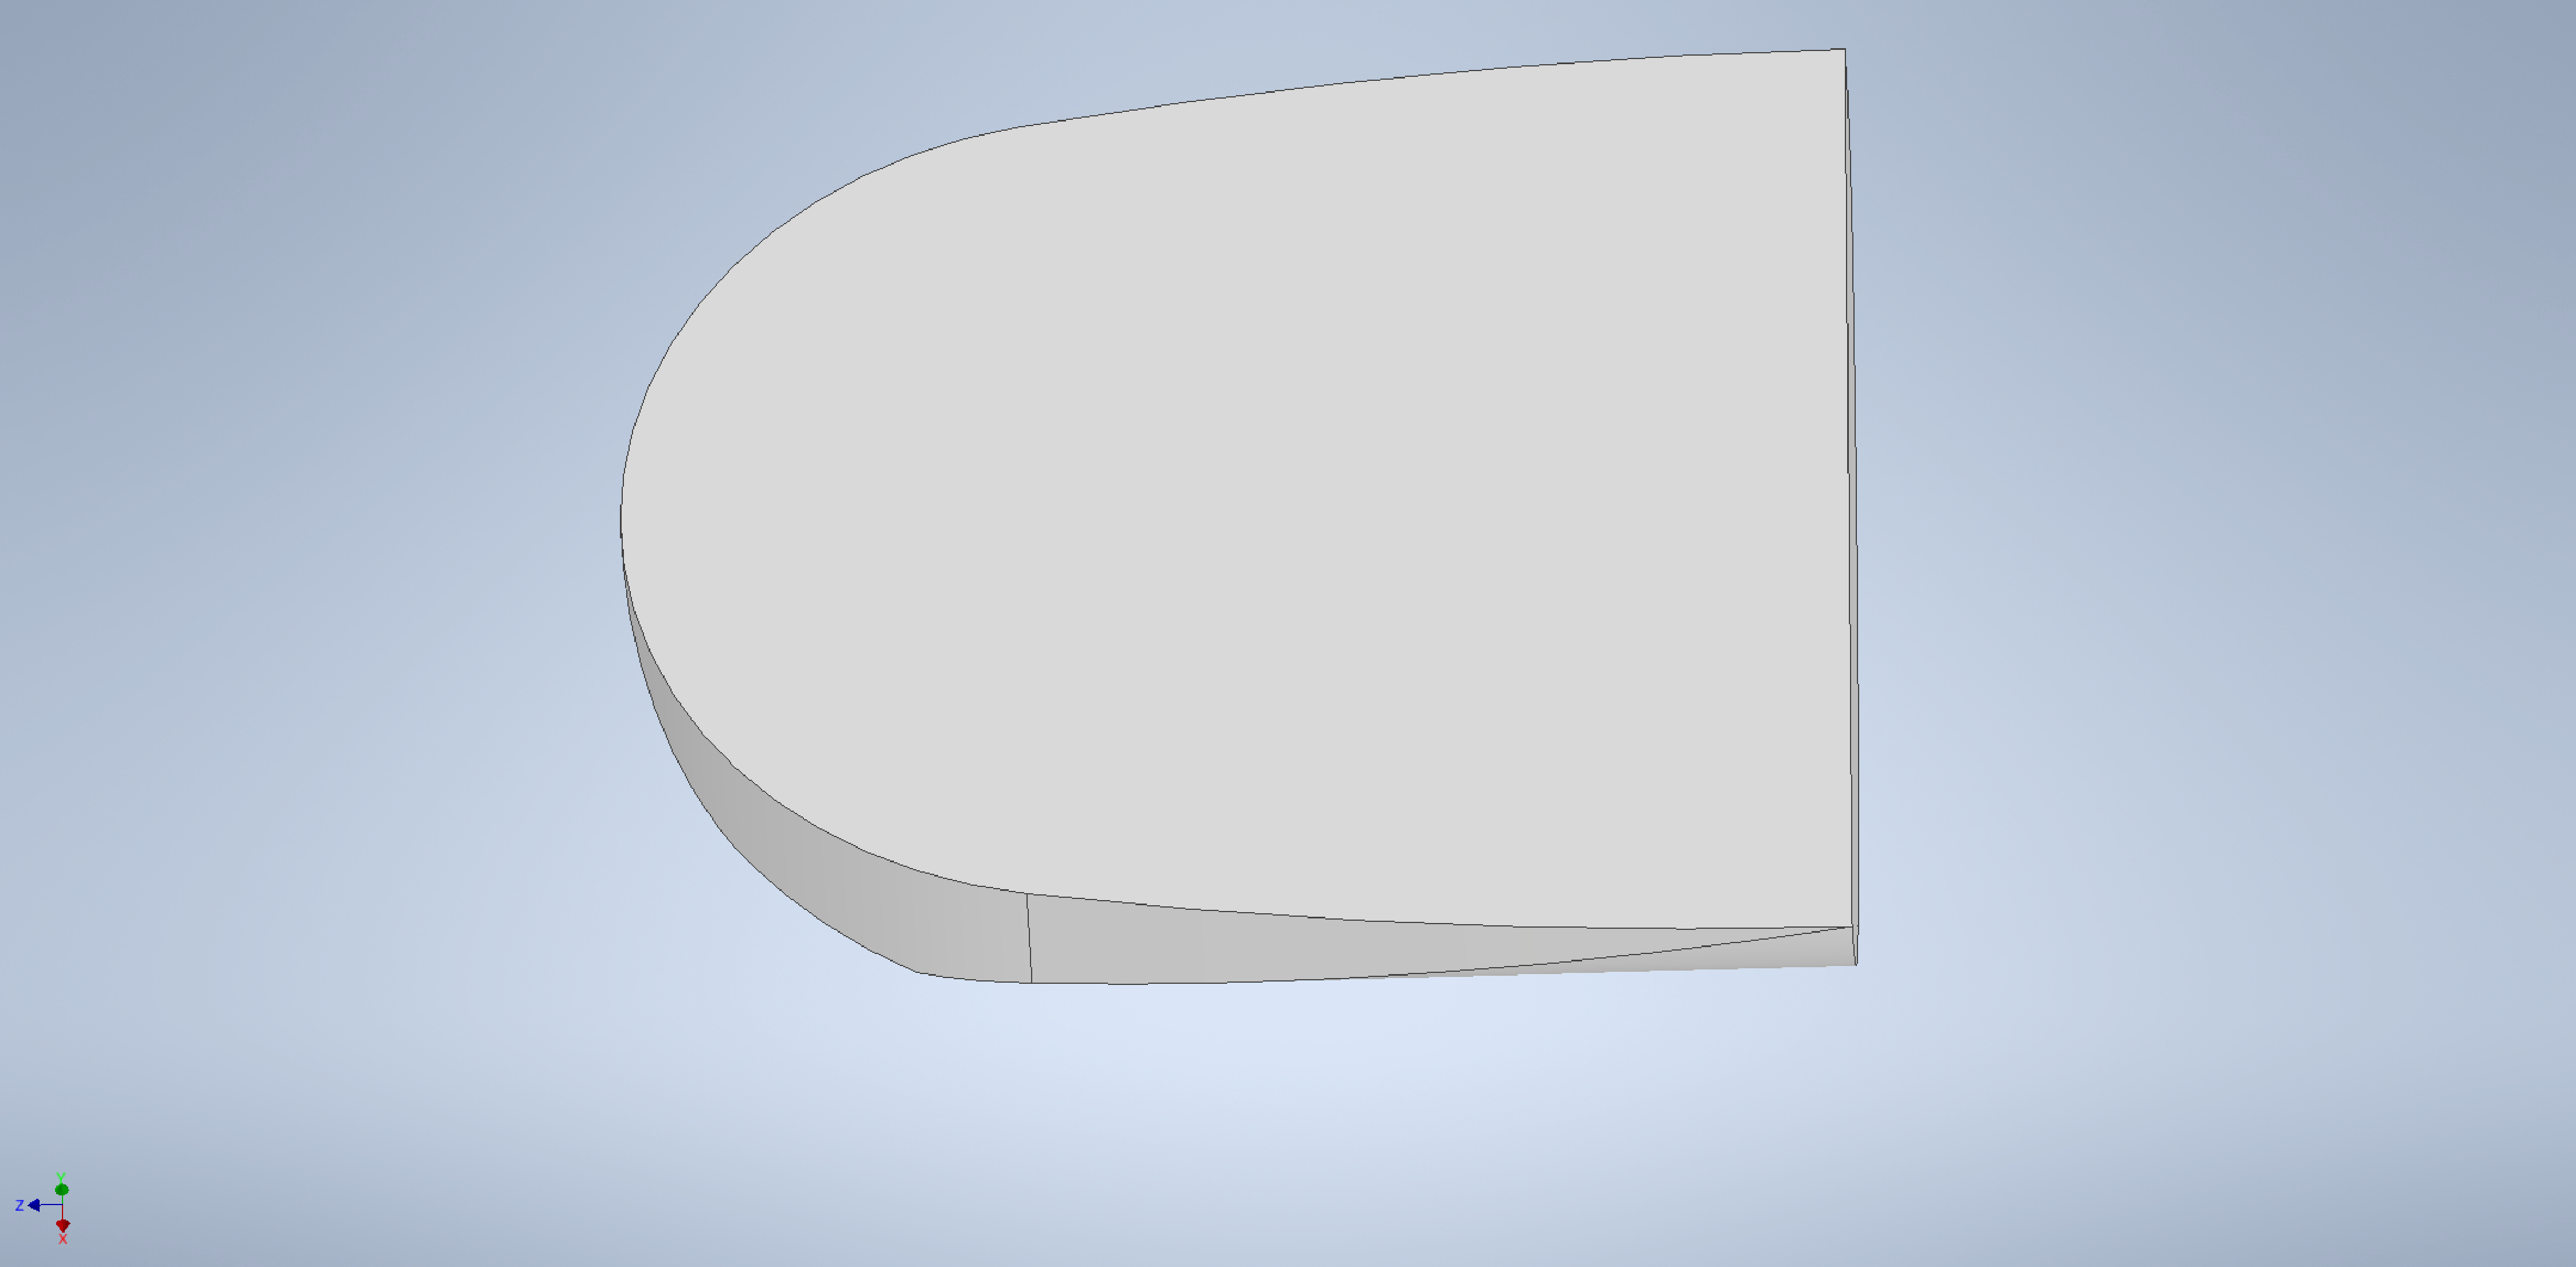
\includegraphics[width=\textwidth]{grundteil.pdf}
	\caption{Grundstruktur eines Einzelteils.}
	\label{img:grundteil}
\end{figure}
\begin{figure}[h]
	\centering
	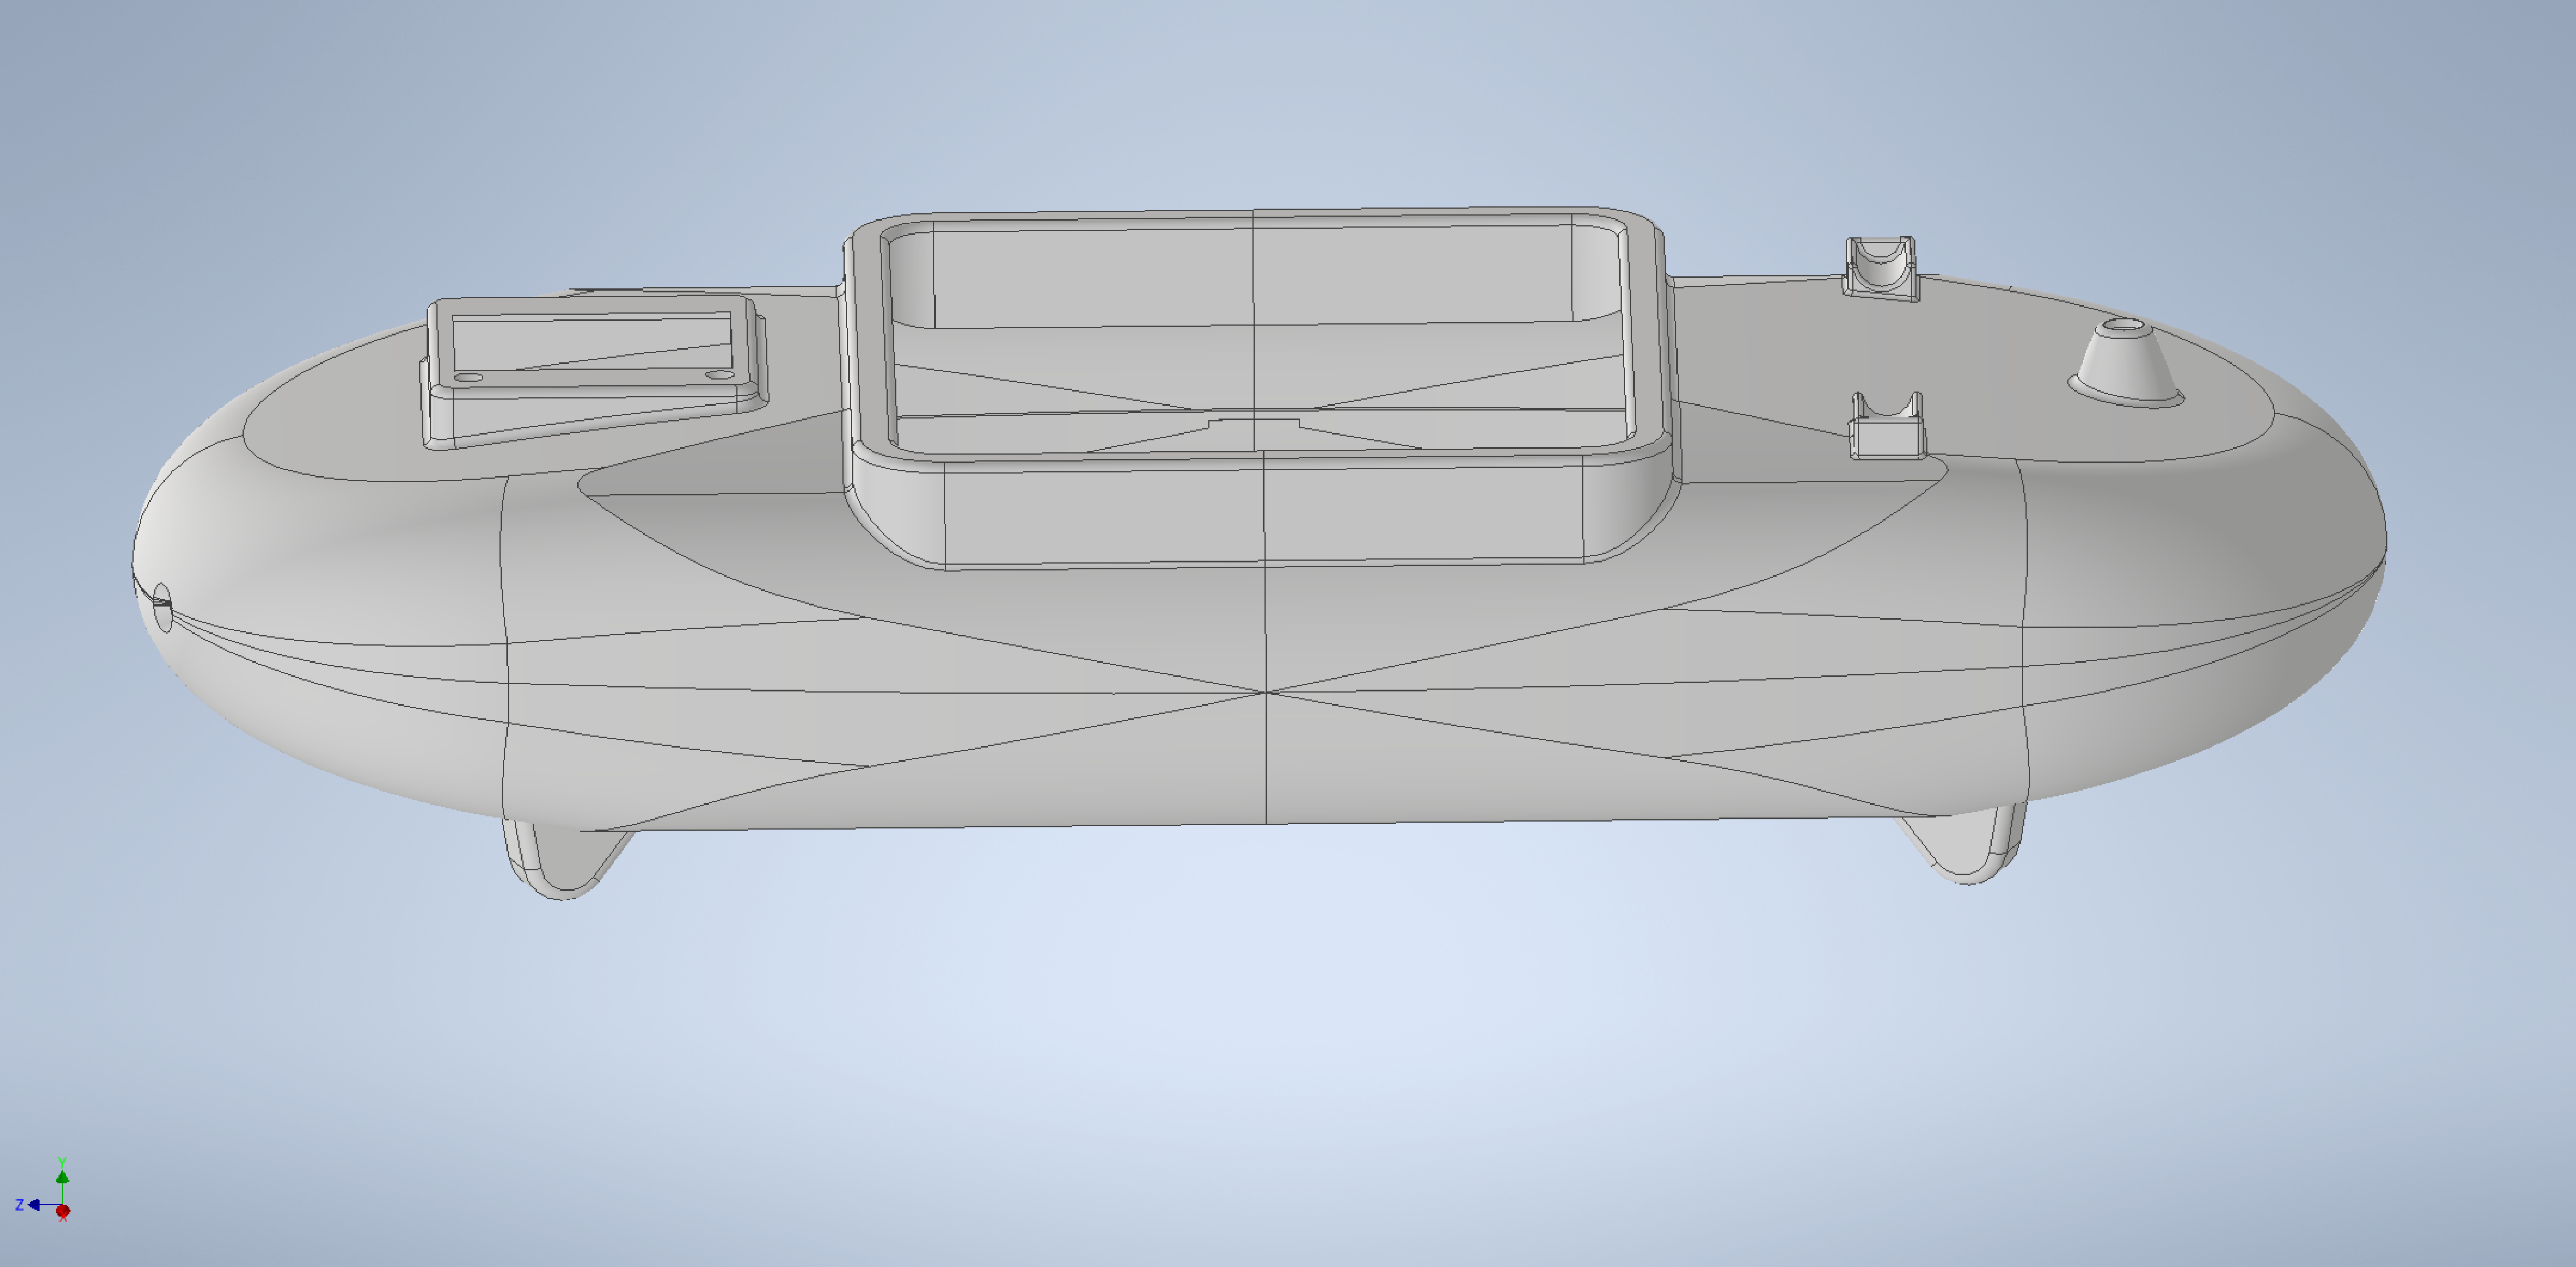
\includegraphics[width=\textwidth]{Theremin_case.pdf}
	\caption{Theremin Gehäuse.}
	\label{img:Theremin_case}
\end{figure}




